\documentclass[10pt]{beamer}

\usetheme[progressbar=frametitle]{metropolis}
\usepackage{appendixnumberbeamer}

\usepackage{booktabs}
\usepackage[scale=2]{ccicons}

\usepackage{pgfplots}
\usepgfplotslibrary{dateplot}

\usepackage{xspace}
\newcommand{\themename}{\textbf{\textsc{metropolis}}\xspace}


% ---
% PACOTES
% --
\usepackage[alf]{abntex2cite}		% Citações padrão ABNT
\usepackage[brazil]{babel}		    % Idioma do documento
\usepackage{color}			       % Controle das cores
\usepackage[T1]{fontenc}		  % Selecao de codigos de fonte.
\usepackage{graphicx}			    % Inclusão de gráficos
\usepackage[utf8]{inputenc}		   % Codificacao do documento (conversão automática dos acentos)
\usepackage{multirow}
\usepackage{threeparttable}
\usepackage[capposition=top]{floatrow}
\usepackage{txfonts}			 % Fontes virtuais
\usepackage{ragged2e}
\usepackage{etoolbox}
\usepackage{lipsum}
\usepackage{amssymb}
% ---

% ---
% Minhas Definições
% ---

%Deixando o Caption alinhado a esquerda mesmo com quebra de linha
\usepackage[labelfont=bf, justification=justified,singlelinecheck=true]{caption}

% Colocando numero de paginas no slide
\setbeamertemplate{footline}[frame number]{}
\setbeamertemplate{caption}[numbered]{}




\title{Relato de Experiência da Criação de Videoaulas sobre Desenvolvimento de Jogos com a Unity}
\date{\today}
% \date{}
\author{Marciano Saraiva e Samy Soares}
\institute{Universidade Federal do Cear\'a - Campus de Quixad\'a}
% \titlegraphic{\hfill\includegraphics[height=1.5cm]{figuras/logo.pdf}}

\begin{document}

\maketitle

\begin{frame}{Roteiro}
	\setbeamertemplate{section in toc}[sections numbered]
	\tableofcontents[hideallsubsections]
\end{frame}

\section{Introdu\c{c}\~ao}

%% ----------------- NOVO SLIDE --------------------------------
\begin{frame}{Introdução}

Os jogos oferecem um mecanismo alternativo de aprendizagem capaz de estimular habilidades de coordenação,
concentração e raciocínio lógico.

Atualmente o mercado de jogos movimenta bilhões de dólares em todo o mundo e é considerado como um mercado ainda em expansão.

\end{frame}


\section{Objetivos}

%% ----------------- NOVO SLIDE --------------------------------
\begin{frame}{Objetivo}

O objetivo dessa atividade é permitir que estudantes de computação pratiquem os conceitos e técnicas aprendidos em sala de aula assim como aumentar o interesse de
estudantes de outras áreas por computação.

\end{frame}

\section{Jogo Desenvolvido}

%% ----------------- NOVO SLIDE --------------------------------
\begin{frame}{Jogo Desenvolvido}

\begin{figure}[H]
	\centering
	\begin{minipage}[b]{0.4\textwidth}
	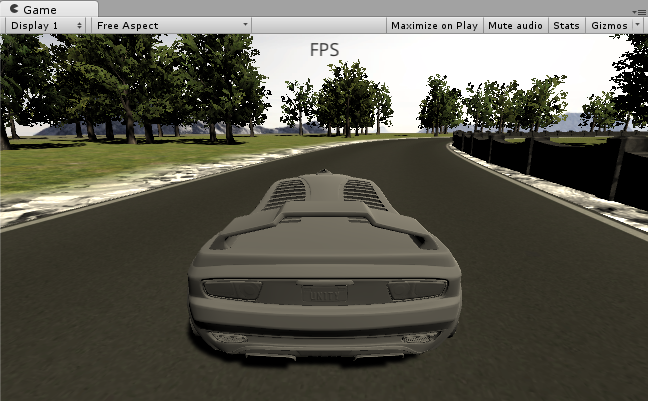
\includegraphics[width=\textwidth]{figuras/game1.png}
	\end{minipage}
	\hfill
	\begin{minipage}[b]{0.4\textwidth}
		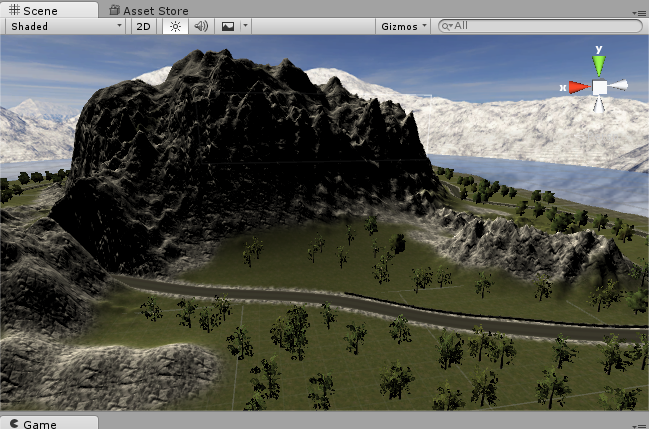
\includegraphics[width=\textwidth]{figuras/game2.png}
	\end{minipage}
\end{figure}

O jogo escolhido como exemplo nas videoaulas foi um jogo de corridas, gênero escolhido por apresentar facilidade de implementação, ser intuitivo aos espectadores,
e permitir explorar mais os recursos da Unity.

\end{frame}

\section{Ferramentas Utilizadas}

%% ----------------- NOVO SLIDE --------------------------------
\begin{frame}{Ferramentas Utilizadas}

\begin{itemize}
		\item Unity 5.3.2
		\item FlashBack Recorder
		\item MonoDevelop
\end{itemize}

\end{frame}


\section{Criação das Videoaulas}

%% ----------------- NOVO SLIDE --------------------------------
\begin{frame}{Criação das Videoaulas}

As primeiras videoaulas possuem caráter introdutório, com a finalidade de apresentar aos espectadores a plataforma de desenvolvimento, seus recursos e
componentes. As aulas seguintes apresentam as etapas da criação do jogo que escolhemos construir.

\begin{itemize}
		\item Criando um Projeto
		\item Novos Objetos, Sistema de Hierarquia e Física
		\item Criando um Terreno
		\item Árvores e Grama
		\item Criando um Carro
		\item Movimentando o Carro
		\item Melhorando a Física do Carro
		\item ...
\end{itemize}

\end{frame}


\section{Públicação do Conteúdo}

%% ----------------- NOVO SLIDE --------------------------------
\begin{frame}{Públicação do Conteúdo}

\begin{figure}[H]
		\centering
		\begin{minipage}[b]{0.7\textwidth}
		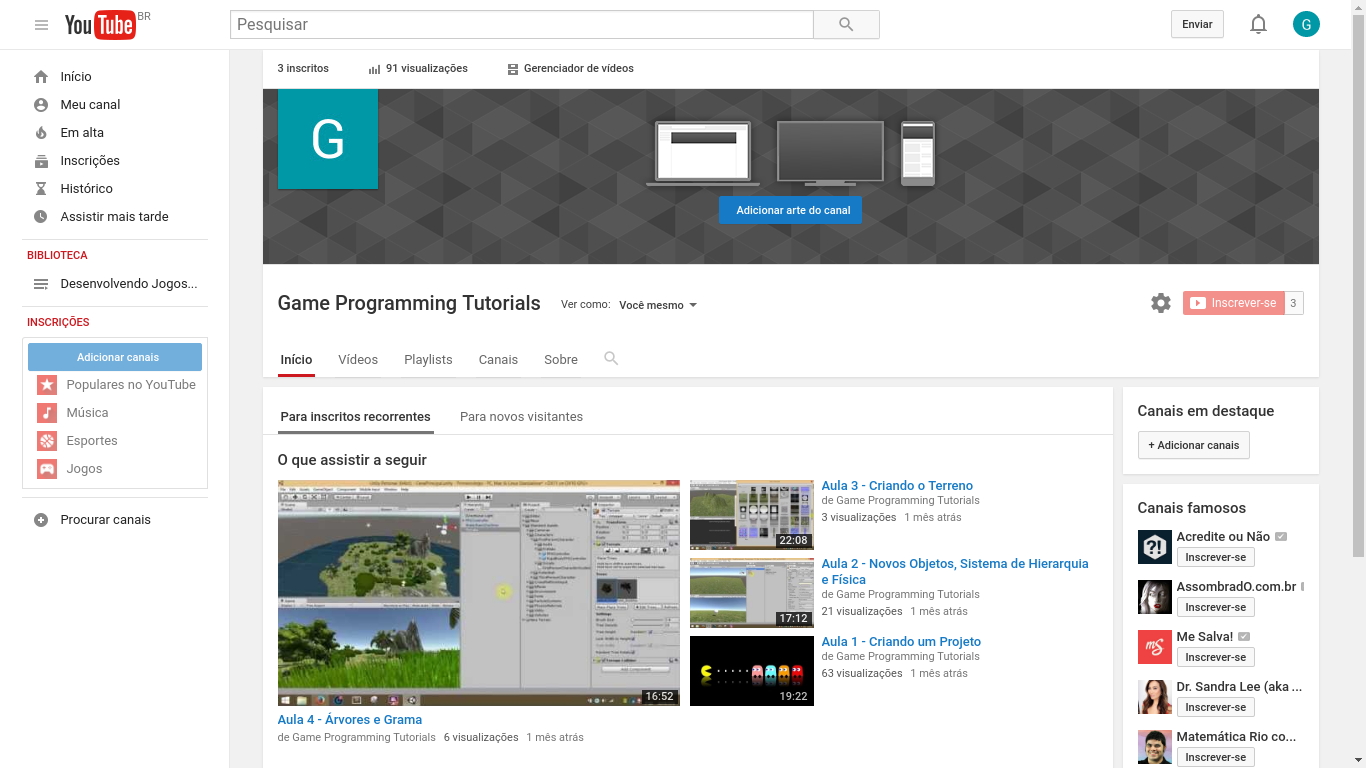
\includegraphics[width=\textwidth]{figuras/publicacao.png}
		\end{minipage}
\end{figure}


Para disponibilizarmos as videoaulas ao público, optamos por criar um canal no YouTube denominado “Game Programming Tutorials”.
Os vídeos estão sendo editados e disponibilizados no canal.

\end{frame}

\section{Lições Aprendidas}

%% ----------------- NOVO SLIDE --------------------------------
\begin{frame}{Lições Aprendidas}

\begin{itemize}
		\item Criando um Projeto
		\item Novos Objetos, Sistema de Hierarquia e Física
		\item Criando um Terreno
		\item Árvores e Grama
		\item Criando um Carro
		\item Movimentando o Carro
		\item Melhorando a Física do Carro
		\item ...
\end{itemize}


\end{frame}


\end{document}
